\documentclass{article}

\usepackage{tikz}

\begin{document}
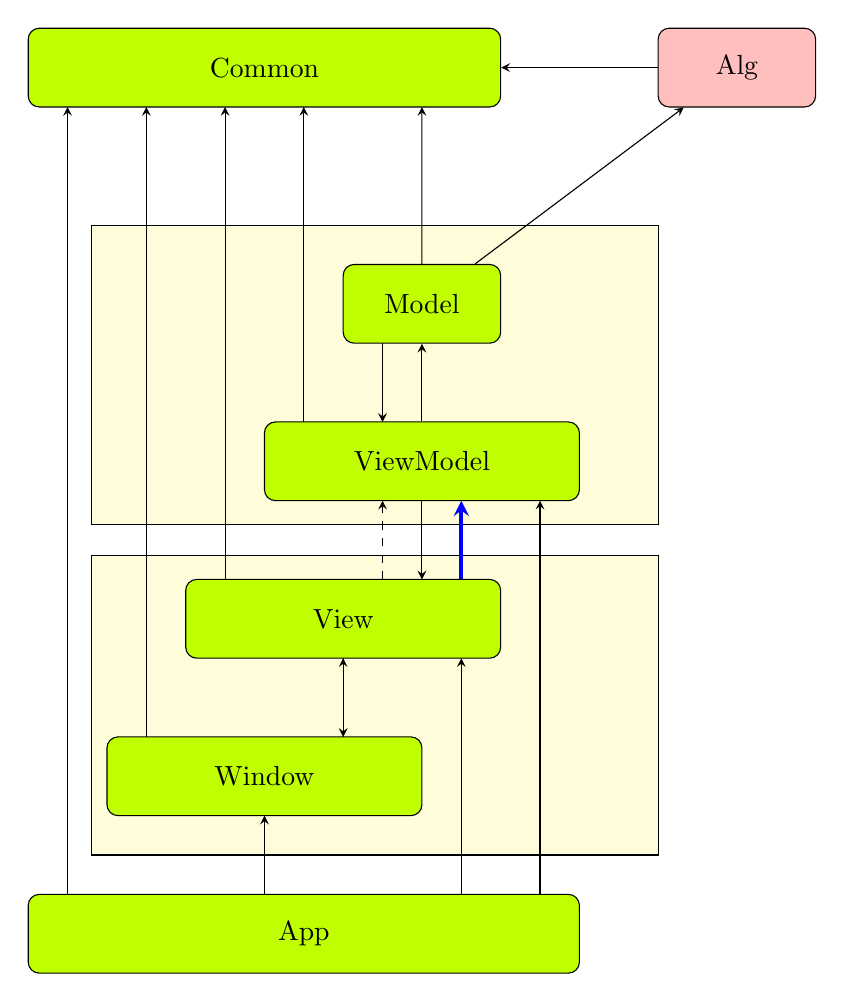
\begin{tikzpicture}
%define
\tikzstyle{state_p} = [rectangle, rounded corners, minimum width=2cm, minimum height=1cm, text centered, draw=black, fill = pink]
\tikzstyle{state_s} = [rectangle, rounded corners, minimum width=2cm, minimum height=1cm, text centered, draw=black, fill = lime]
\tikzstyle{state_m} = [rectangle, rounded corners, minimum width=4cm, minimum height=1cm, text centered, draw=black, fill = lime]
\tikzstyle{state_l} = [rectangle, rounded corners, minimum width=6cm, minimum height=1cm, text centered, draw=black, fill = lime]
\tikzstyle{state_xl} = [rectangle, rounded corners, minimum width=7cm, minimum height=1cm, text centered, draw=black, fill = lime]
\tikzstyle{arrow} = [->, >=stealth]
\tikzstyle{arrowb} = [->, >=stealth, blue, line width = 0.05cm]
\tikzstyle{arrowx} = [->, >=stealth, dashed]

%block1
\filldraw[fill = yellow, opacity = 0.15, draw opacity = 1](-2.2,-2)rectangle(5,-5.8);
%block2
\filldraw[fill = yellow, opacity = 0.15, draw opacity = 1](-2.2,-6.2)rectangle(5,-10);

\node[state_l, draw, align=left](state_Common){Common};
\node[state_p, right of = state_Common, xshift = 5cm, draw, align=left](state_Alg){Alg};
\node[state_s, below of = state_Common, xshift = 2cm, yshift = -2cm, draw, align=left](state_Model){Model};
\node[state_m, below of = state_Common, xshift = 2cm, yshift = -4cm, draw, align=left](state_VM){ViewModel};
\node[state_m, below of = state_Common, xshift = 1cm, yshift = -6cm, draw, align=left](state_View){View};
\node[state_m, below of = state_Common, yshift = -8cm, draw, align=left](state_Window){Window};
\node[state_xl, below of = state_Common, xshift = 0.5cm, yshift = -10cm, draw, align=left](state_App){App};
%line
\draw[arrow](state_Model)--(state_Alg);
\draw[arrow](state_Alg)--(state_Common);
\draw[arrow](state_Model)--(2,-0.5); %Model->Common
\draw[arrow](0.5,-4.5)--(0.5,-0.5); %ViewModel->Common
\draw[arrow](-0.5,-6.5)--(-0.5,-0.5); %View->Common
\draw[arrow](-1.5,-8.5)--(-1.5,-0.5); %Window->Common
\draw[arrow](-2.5,-10.5)--(-2.5,-0.5); %App->Common
\draw[arrow](1.5,-3.5)--(1.5,-4.5); %Model->ViewModel
\draw[arrow](state_VM)--(state_Model);
\draw[arrowx](1.5,-6.5)--(1.5,-5.5); %View->ViewModel
\draw[arrow](2,-5.5)--(2,-6.5); %ViewModel->View
\draw[arrowb](2.5,-6.5)--(2.5,-5.5); %View->ViewModel(blue)
\draw[arrow](1,-7.5)--(1,-8.5); %View<->Window
\draw[arrow](1,-8.5)--(1,-7.5);
\draw[arrow](0,-10.5)--(0,-9.5); %App->Window
\draw[arrow](2.5,-10.5)--(2.5,-7.5); %App->View
\draw[arrow](3.5,-10.5)--(3.5,-5.5); %App->ViewModel

\end{tikzpicture}
\end{document}